\documentclass[]{report}
\usepackage{indentfirst}
\usepackage{listings}
\usepackage[svgnames]{xcolor}
\usepackage{graphicx}


\graphicspath{{./}}

\lstdefinestyle{mstyle}{
	frame=lines,
	showlines=false,
	showspaces=false,
	showstringspaces=false,
	basicstyle=\ttfamily\footnotesize,
	%prebreak = \raisebox{0ex}[0ex][0ex]{\ensuremath{\hookleftarrow}},
	backgroundcolor=\color{WhiteSmoke}, % set backgroundcolor
	breakatwhitespace=false,
	captionpos=b,
	keepspaces=true,
	numbers=left,
	numberstyle=\ttfamily \color{DarkCyan},
	numbersep=5pt,
	keywordstyle=\color{Chocolate},
	identifierstyle=\ttfamily \color{MediumVioletRed},
	stringstyle=\color{MediumBlue},
	commentstyle=\color{DarkGreen},
	breaklines=true,
	tabsize=4,
	rulecolor=\color{Teal}
}

%\lstset{language=Gnuplot,
%	frame=lines,
%	showlines=false,
%	showspaces=false,
%	showstringspaces=false,
%	basicstyle=\ttfamily\footnotesize,
%	backgroundcolor=\color{WhiteSmoke}, % set backgroundcolor
%	breakatwhitespace=false,
%	captionpos=b,
%	keepspaces=true,
%	numbers=left,
%	numberstyle=\ttfamily \color{DarkCyan},
%	numbersep=5pt,
%	keywordstyle=\color{Chocolate},
%	identifierstyle=\ttfamily \color{MediumVioletRed},
%	stringstyle=\color{MediumBlue},
%	commentstyle=\color{DarkGreen},
%	breaklines=true,
%	tabsize=2,
%	rulecolor=\color{Teal}
%}

% Title Page
\title{Computational Modeling of Leonard Jones Fluid}
\author{Apratim Rastogi}
\date{}

\begin{document}
\maketitle
\pagenumbering{arabic}

\begin{abstract}
	This is a report on computational modeling of Leonard Jones fluid using Monte Carlo Metropolis algorithm with periodic boundary condition. In this report I have tried to simulate the relation between pressure and density of a randomly configured Leonard Jones fluid at two different temperature. I have provided the code implemented in C++ with the Gnuplot script for plotting and simulating the system.  
\end{abstract}
\section*{Method used}
	The current project was done using metropolis algorithm which is a type of Monte Carlo simulation method. The system taken is a 2D Leonard Jones fluid (section 0.2) in a continuous space with periodic boundary conditions.
	
\paragraph*{Monte Carlo Metropolis algorithm}
	Monte Carlo simulation also known as Monte Carlo Method is a mathematical algorithm that calculates the likelihood of range of results by repeated random sampling. This method was developed by John Von N	eumann and Stainslaw Ulma during Manhattan Project to improve decision making under uncertain circumstances. Monte Carlo Simulation predicts a set of outcomes based on an estimated range of values versus a set of fixed input values. In other words, a Monte Carlo Simulation builds a model of possible results by leveraging a probability distribution, such as a uniform or normal distribution, for any variable that has inherent uncertainty. It, then, recalculates the results over and over, each time using a different set of random numbers between the minimum and maximum values. In a typical Monte Carlo experiment, this exercise can be repeated thousands of times to produce a large number of likely outcomes.\paragraph{}
	 The Metropolis algorithm is a special case of an importance-sampling procedure in which certain possible sampling attempts are rejected. The Metropolis method is useful for computing averages of the form \[{<f> =\frac{\int f(x)p(x)dx}{\int p(x)dx}}\] The Metropolis algorithm produces a random walk of	points ${xi}$ whose asymptotic probability distribution approaches $p(x)$ after a large number of steps. The random walk is defined by specifying a transition probability $T (xi \rightarrow xj )$ from one value xi to another value xj such that the distribution of points x0 , x1, x2, . . . converges to $p(x)$. The relation does not specify $T (xi \rightarrow xj )$ uniquely. A simple choice of $T (xi \rightarrow xj )$ that is consistent with is \[  T (xi \rightarrow xj ) = \min[1,\frac{p(x_j)}{p(x_i)}] \]

\section*{Leonard Jones Simulation}
	Leonard Jones Potential is a simplified model of particles in a fluid which nonetheless describes the essential properties of how particles interact in a fluid. Primary objective of this simulation is to predict the pressure of given sample of Leonard Jones fluid given density and temperature. We assume certain number of particles N (depending upon the hardware and given time we set it) and Density $\rho$ and Temperature T. In this case we have taken 100 particles for all runs with $\rho$ varying in range 0.1-1 with intervals of 0.1 and we have run this for T=2 K and T=0.9 K. \paragraph{}
	Pressure is computed by \[P = \rho T + vir/V \] where vir(for two dimensions) is \[vir = \frac{1}{2}\sum f(r_{ij}).r_{ij}\] and V is the system volume calculated by \[V = \frac{N}{\rho}\]
	Leonard Jones pair potential is calculated by 
	\[ \frac{\partial u(r_{ij})}{\partial r_{ij}} = 4*[-12\frac{\sigma^{12}}{r^{13}_{ij}} + 6\frac{\sigma^{6}}{r^{7}_{ij}}]\]
	so, 
	\[ \textbf{f}(r_{ij}) = \frac{r_{ij}}{r_{ij}^2}  \big\{ 48 \big[\left(\frac{\sigma}{r_{ij}} \right)^{12} + \frac{1}{2} \left( \frac{\sigma}{r_{ij}} \right)^6 \big] \big\} \]
	Finally, therefore virial is, 
	\[ vir = \frac{1}{2} \sum_{i<j}  \big\{48\big[\left(\frac{\sigma}{r_{ij}} \right)^{12} + \frac{1}{2} \left( \frac{\sigma}{r_{ij}} \right)^6  \big] \big\} \]
	Notice that any particular pair's contribution to the total virial is positive if the members of the pair are repelling one another (positive $f$ along ${\bf r}_{ij}$), and negative if the particles are attracting one another.
	
	Given below is the code for simulating this in C++ and gnuplot script I've used to graphically simulate it.
\newpage	
\subsection*{C++ code for the simulation}
\begin{lstlisting}[language=C++,style=mstyle]
#include <iostream>
#include <cstdlib>
#include <cmath>
#include <fstream>

#define myrand() (rand()/double(RAND_MAX))//defining uniform random number generator
using namespace std;

//Engergy calculation
double energy(double * xx, double *yy,double &vir,int N,double L)
{double r2,r6,e=0.0,dx,dy,hL=L/2.0;
vir =0.0;
	for(int i=0; i<N; i++)
	{
		for(int j=i+1;j<N;j++)
		{
			dx = xx[i]-xx[j];
			dy = yy[i]-yy[j];
			
			//boundary conditions
			if (dx>hL)       dx-=L;
			else if (dx<-hL) dx+=L;
			if (dy>hL)       dy-=L;
			else if (dy<-hL) dy+=L;
				
			r2 = dx*dx + dy*dy; // r is the distance
			r6 = 1.0/(r2*r2*r2); // calculating r^6 
			e += 4*(r6*r6 - r6);
			vir += 24*(r6*r6-0.5*r6);   //Calculating virial
			
		}
	}
	return e;
}
	
//Initialize the configuration
void init(double * xx, double *yy, double L,int N) 
{int c = 0,n=sqrt(N);
	cout<< N<<" "<<n<<endl;
	cout<< L<<endl;
	double d= L/n; //lattice constant 
	cout<< d<<endl;
	
	for(int i=0; i<n;i++)
	{
		for(int j=0;j<n;j++)
		{
			xx[c]=j*d;
			yy[c]=i*d;
			c++;
		}
	}
}
	
//Metrolpolis Algorithm
double metropolis(double * xx,double *yy,double V,double rho,int cycle,int N,double L,double T,ofstream& fp,double *p_c)
{
	int pr;
	double x_old, y_old, E_old, E_new,dr=0.1,dx,dy;
	double racc,facc=0.0;
	double vir_new=0.0,vir_old=0.0,vir_sum=0.0,p,p_sum=0.0;
	E_old = energy(xx,yy,vir_old,N,L);
		
	ofstream simf("LJ_sim.txt"); //File for simulating the states of the system
		
		
	for(int c=0;c<cycle; c++)
	{
		for(int id=0;id<N;id++)
		{
			pr = myrand()*N; //randomly choose a particle by its index
			
			// Record the previous positions
			x_old=xx[pr];
			y_old=yy[pr];
			
			dx = dr*(2*myrand()-1);
			dy = dr*(2*myrand()-1);
			
			xx[pr] += dx;
			yy[pr] += dy;
				
			//Apply periodic boundary conditions
			if(xx[pr]<0.0) xx[pr]+=L;
			if(xx[pr]>L) xx[pr]-=L;
			if(yy[pr]<0.0) yy[pr]+=L;
			if(yy[pr]>L) yy[pr]-=L;
			
			
			E_new = energy(xx,yy,vir_new,N,L);
				
			if(myrand()<exp(-T*(E_new-E_old)))
			{
				E_old=E_new;
				vir_old = vir_new;
				facc +=1;
			}
			else
			{
				xx[pr]=x_old;
				yy[pr]=y_old;
			}
				
			simf << xx[id]<<" "<<yy[id]<<"\n";
		}
			
		//Adjusting maximum displacement according to the system parameters
		racc = facc/N;
		if (racc >0.5)
		{dx *= 1.05;dy *= 1.05;}
		else {dx *= 0.95;dy *= 0.95;}
		
		simf <<"\n"<<"\n";
			
		p = rho*(T)+vir_old/V;
		p_c[c] = p;
			
		// Cycle vs Energy plot
		fp << c<<" "<<(E_old/N)<<" "<<p<<endl;
		cout << c << " "<<(E_old/N)<<" "<<p<<endl;
		
		if(c>5000 && c%100==0)
		{p_sum += p;}
		
		
	}
	simf.close();
		
	return (p_sum/(cycle-5000));
}
	
double correlation(double *p,int N, int t) //Calculating correlation of pressure
{
	//C(t) = (<s(T)s(T+t)> - <s(T)>)/(<s^2(T)> - <s(T)>^2);
	double p_sum=0,p2_sum=0,pt_sum=0,p_avg,cor;
	for(int i=0; i<N; i++)
	{
		p_sum += p[i];
		p2_sum += p[i]*p[i];
		if ((i+t) > N) continue;
		pt_sum += p[i]*p[i+t];
			
	}
	p_avg = p_sum/N;
	cor = (pt_sum/(N-t) -p_avg*p_avg)/(p2_sum/N - p_avg*p_avg);
		
	return cor;
}
	
	
int main()
{
		
int cycle=10000;
int N=10*10;  // NUmber of particles = 100
double T,V,L,rho,p_avg;
double xx[N],yy[N];
	
//array to store pressure so to calculate correlation afterwards
double p_c[cycle];
		
cout << "Enter the temperature"<<endl;
//cin >> T;
T = 2;
T = 1/T;// reciprocal of Temperature for efficiency
rho = 0.5;
V = N/rho; //Volume = N/rho 
L = sqrt(V);
	
	
ofstream fp("Energy.txt");
	
init(xx,yy,L,N);
cout<<"OKAY"<<endl;
p_avg = metropolis(xx,yy,V,rho,cycle,N,L,T,fp,p_c);
	
fp.close();
		
cout<<"Pressure: "<<p_avg<<"\nDensity: "<<rho<<endl;
cout<<"Temperature: "<<T<<endl;
	
	
//Ploting the energy graph using gnuplot 
FILE* gnuplot;
gnuplot = popen("gnuplot -p", "w");
if(gnuplot != NULL)
{fprintf(gnuplot, "p 'Energy.txt' usi 1:3 w l\n");}
fprintf(gnuplot, "p 'Energy.txt' usi 1:2 w l \n");s
//fprintf(gnuplot, "p 'Energy.txt' usi 1:3\n");

//Simulation of the system using gnuplot script
system("gnuplot LJ_simulation.gnu");
ofstream fcor("correlation.txt");
		
double cor;
for(int i=1; i<100; i++)
{
	fcor<<i<<" "<<correlation(p_c,N,i)<<endl;
}
		
fcor.close();
return 0;
}
\end{lstlisting}

\subsection*{Gnuplot code for simulation}
\begin{lstlisting}[language=Gnuplot,style=mstyle]
	reset
	T=10000
	set xrange[0:16]
	set yrange[0:16]
	do for[t=0:T]{
		p 'LJ_sim.txt' i t w p pt 7 ps 1.26 lc 'red'
		set title sprintf("Time t=%d",t)
		#pause 0.01
	}
\end{lstlisting}

\newpage
\subsection*{Pressure Vs Density Graph at two different temperatures}
\begin{figure}[h] 
	\centering 
	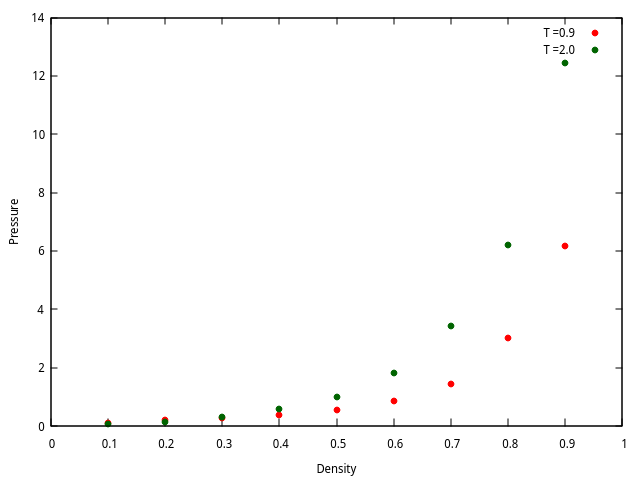
\includegraphics[scale=0.8]{Pressure vs Density graph}
	\caption{ This graph shows how average pressure was changing with as the density of the fluid increased. The red dots shows $P$ vs $\rho$ for $T=0.9$ and blue dots shows for $T=2.0$}
		
\end{figure}
The above result is achieved by running 10000 cycles for each Density and Temperature with system size of 100 particles in 2-D space (Results might slightly vary for 3-D space).

\newpage
\subsection*{Auto-Correlation Graph for pressure}
\begin{figure}[h]
	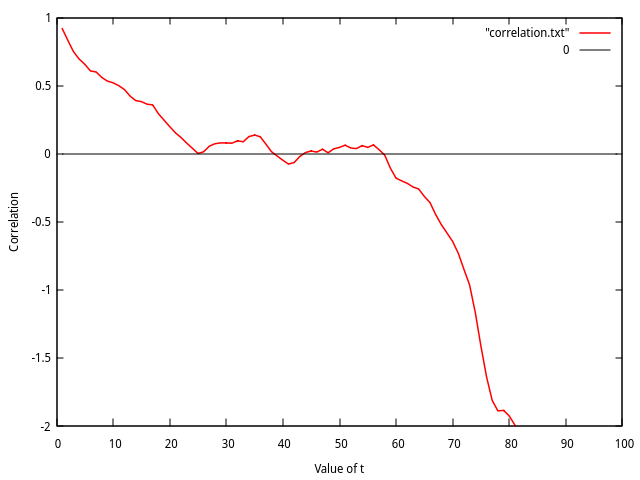
\includegraphics[scale=0.8]{Correlation graph}
	\caption{ This graph shows the correlation between data taken once for $T=2$ and $\rho=0.5$(although tested for many data sets)}
\end{figure}
I have used auto-correlation function to find the correlation between data (for pressure in this particular case). For the given system size of 100 particles, a good amount of correlation can be seen in the data. As it can be seen from the graph, the correlation approaches to 0 when t = 60 (t is the lag value between data pairs) therefore, just to be safe, I have a averaged the data from above simulation after ever 100 data points.

\newpage
\section*{Conclusion}
This report states the relationship between Density and Pressure for a given Temperature of a Leonard Jones Fluid

\section*{References}

\begin{enumerate}
	\item @book{0805377581, 9780805377583,
		author = {Harvey Gould, Jan Tobochnik, and Wolfgang Christian},
		title = {An Introduction to Computer Simulation Methods
			Applications to Physical System},
		date = {August 27, 2016}.}
	\item @online{author = {Cameron Abrams}, title = {Case Study 4 (F and S Case Study 1): Equation of State of the Lennard-Jones Fluid},
		date = {March 13, 2013},
		url = {http://www.pages.drexel.edu/~cfa22/msim/node19.html}. }
	
	
	
\end{enumerate}



\end{document}          
